% Options for packages loaded elsewhere
\PassOptionsToPackage{unicode}{hyperref}
\PassOptionsToPackage{hyphens}{url}
\PassOptionsToPackage{dvipsnames,svgnames,x11names}{xcolor}
%
\documentclass[
  10pt,
  letterpaper,
  DIV=11,
  numbers=noendperiod]{scrartcl}

\usepackage{amsmath,amssymb}
\usepackage{iftex}
\ifPDFTeX
  \usepackage[T1]{fontenc}
  \usepackage[utf8]{inputenc}
  \usepackage{textcomp} % provide euro and other symbols
\else % if luatex or xetex
  \usepackage{unicode-math}
  \defaultfontfeatures{Scale=MatchLowercase}
  \defaultfontfeatures[\rmfamily]{Ligatures=TeX,Scale=1}
\fi
\usepackage{lmodern}
\ifPDFTeX\else  
    % xetex/luatex font selection
\fi
% Use upquote if available, for straight quotes in verbatim environments
\IfFileExists{upquote.sty}{\usepackage{upquote}}{}
\IfFileExists{microtype.sty}{% use microtype if available
  \usepackage[]{microtype}
  \UseMicrotypeSet[protrusion]{basicmath} % disable protrusion for tt fonts
}{}
\makeatletter
\@ifundefined{KOMAClassName}{% if non-KOMA class
  \IfFileExists{parskip.sty}{%
    \usepackage{parskip}
  }{% else
    \setlength{\parindent}{0pt}
    \setlength{\parskip}{6pt plus 2pt minus 1pt}}
}{% if KOMA class
  \KOMAoptions{parskip=half}}
\makeatother
\usepackage{xcolor}
\usepackage[left = 2.5cm, righ t= 2.5cm, top = 3cm, bottom =
3cm]{geometry}
\setlength{\emergencystretch}{3em} % prevent overfull lines
\setcounter{secnumdepth}{-\maxdimen} % remove section numbering
% Make \paragraph and \subparagraph free-standing
\makeatletter
\ifx\paragraph\undefined\else
  \let\oldparagraph\paragraph
  \renewcommand{\paragraph}{
    \@ifstar
      \xxxParagraphStar
      \xxxParagraphNoStar
  }
  \newcommand{\xxxParagraphStar}[1]{\oldparagraph*{#1}\mbox{}}
  \newcommand{\xxxParagraphNoStar}[1]{\oldparagraph{#1}\mbox{}}
\fi
\ifx\subparagraph\undefined\else
  \let\oldsubparagraph\subparagraph
  \renewcommand{\subparagraph}{
    \@ifstar
      \xxxSubParagraphStar
      \xxxSubParagraphNoStar
  }
  \newcommand{\xxxSubParagraphStar}[1]{\oldsubparagraph*{#1}\mbox{}}
  \newcommand{\xxxSubParagraphNoStar}[1]{\oldsubparagraph{#1}\mbox{}}
\fi
\makeatother

\usepackage{color}
\usepackage{fancyvrb}
\newcommand{\VerbBar}{|}
\newcommand{\VERB}{\Verb[commandchars=\\\{\}]}
\DefineVerbatimEnvironment{Highlighting}{Verbatim}{commandchars=\\\{\}}
% Add ',fontsize=\small' for more characters per line
\usepackage{framed}
\definecolor{shadecolor}{RGB}{241,243,245}
\newenvironment{Shaded}{\begin{snugshade}}{\end{snugshade}}
\newcommand{\AlertTok}[1]{\textcolor[rgb]{0.68,0.00,0.00}{#1}}
\newcommand{\AnnotationTok}[1]{\textcolor[rgb]{0.37,0.37,0.37}{#1}}
\newcommand{\AttributeTok}[1]{\textcolor[rgb]{0.40,0.45,0.13}{#1}}
\newcommand{\BaseNTok}[1]{\textcolor[rgb]{0.68,0.00,0.00}{#1}}
\newcommand{\BuiltInTok}[1]{\textcolor[rgb]{0.00,0.23,0.31}{#1}}
\newcommand{\CharTok}[1]{\textcolor[rgb]{0.13,0.47,0.30}{#1}}
\newcommand{\CommentTok}[1]{\textcolor[rgb]{0.37,0.37,0.37}{#1}}
\newcommand{\CommentVarTok}[1]{\textcolor[rgb]{0.37,0.37,0.37}{\textit{#1}}}
\newcommand{\ConstantTok}[1]{\textcolor[rgb]{0.56,0.35,0.01}{#1}}
\newcommand{\ControlFlowTok}[1]{\textcolor[rgb]{0.00,0.23,0.31}{\textbf{#1}}}
\newcommand{\DataTypeTok}[1]{\textcolor[rgb]{0.68,0.00,0.00}{#1}}
\newcommand{\DecValTok}[1]{\textcolor[rgb]{0.68,0.00,0.00}{#1}}
\newcommand{\DocumentationTok}[1]{\textcolor[rgb]{0.37,0.37,0.37}{\textit{#1}}}
\newcommand{\ErrorTok}[1]{\textcolor[rgb]{0.68,0.00,0.00}{#1}}
\newcommand{\ExtensionTok}[1]{\textcolor[rgb]{0.00,0.23,0.31}{#1}}
\newcommand{\FloatTok}[1]{\textcolor[rgb]{0.68,0.00,0.00}{#1}}
\newcommand{\FunctionTok}[1]{\textcolor[rgb]{0.28,0.35,0.67}{#1}}
\newcommand{\ImportTok}[1]{\textcolor[rgb]{0.00,0.46,0.62}{#1}}
\newcommand{\InformationTok}[1]{\textcolor[rgb]{0.37,0.37,0.37}{#1}}
\newcommand{\KeywordTok}[1]{\textcolor[rgb]{0.00,0.23,0.31}{\textbf{#1}}}
\newcommand{\NormalTok}[1]{\textcolor[rgb]{0.00,0.23,0.31}{#1}}
\newcommand{\OperatorTok}[1]{\textcolor[rgb]{0.37,0.37,0.37}{#1}}
\newcommand{\OtherTok}[1]{\textcolor[rgb]{0.00,0.23,0.31}{#1}}
\newcommand{\PreprocessorTok}[1]{\textcolor[rgb]{0.68,0.00,0.00}{#1}}
\newcommand{\RegionMarkerTok}[1]{\textcolor[rgb]{0.00,0.23,0.31}{#1}}
\newcommand{\SpecialCharTok}[1]{\textcolor[rgb]{0.37,0.37,0.37}{#1}}
\newcommand{\SpecialStringTok}[1]{\textcolor[rgb]{0.13,0.47,0.30}{#1}}
\newcommand{\StringTok}[1]{\textcolor[rgb]{0.13,0.47,0.30}{#1}}
\newcommand{\VariableTok}[1]{\textcolor[rgb]{0.07,0.07,0.07}{#1}}
\newcommand{\VerbatimStringTok}[1]{\textcolor[rgb]{0.13,0.47,0.30}{#1}}
\newcommand{\WarningTok}[1]{\textcolor[rgb]{0.37,0.37,0.37}{\textit{#1}}}

\providecommand{\tightlist}{%
  \setlength{\itemsep}{0pt}\setlength{\parskip}{0pt}}\usepackage{longtable,booktabs,array}
\usepackage{calc} % for calculating minipage widths
% Correct order of tables after \paragraph or \subparagraph
\usepackage{etoolbox}
\makeatletter
\patchcmd\longtable{\par}{\if@noskipsec\mbox{}\fi\par}{}{}
\makeatother
% Allow footnotes in longtable head/foot
\IfFileExists{footnotehyper.sty}{\usepackage{footnotehyper}}{\usepackage{footnote}}
\makesavenoteenv{longtable}
\usepackage{graphicx}
\makeatletter
\def\maxwidth{\ifdim\Gin@nat@width>\linewidth\linewidth\else\Gin@nat@width\fi}
\def\maxheight{\ifdim\Gin@nat@height>\textheight\textheight\else\Gin@nat@height\fi}
\makeatother
% Scale images if necessary, so that they will not overflow the page
% margins by default, and it is still possible to overwrite the defaults
% using explicit options in \includegraphics[width, height, ...]{}
\setkeys{Gin}{width=\maxwidth,height=\maxheight,keepaspectratio}
% Set default figure placement to htbp
\makeatletter
\def\fps@figure{htbp}
\makeatother

\KOMAoption{captions}{tableheading}
\makeatletter
\@ifpackageloaded{caption}{}{\usepackage{caption}}
\AtBeginDocument{%
\ifdefined\contentsname
  \renewcommand*\contentsname{Tabla de contenidos}
\else
  \newcommand\contentsname{Tabla de contenidos}
\fi
\ifdefined\listfigurename
  \renewcommand*\listfigurename{Listado de Figuras}
\else
  \newcommand\listfigurename{Listado de Figuras}
\fi
\ifdefined\listtablename
  \renewcommand*\listtablename{Listado de Tablas}
\else
  \newcommand\listtablename{Listado de Tablas}
\fi
\ifdefined\figurename
  \renewcommand*\figurename{Figura}
\else
  \newcommand\figurename{Figura}
\fi
\ifdefined\tablename
  \renewcommand*\tablename{Tabla}
\else
  \newcommand\tablename{Tabla}
\fi
}
\@ifpackageloaded{float}{}{\usepackage{float}}
\floatstyle{ruled}
\@ifundefined{c@chapter}{\newfloat{codelisting}{h}{lop}}{\newfloat{codelisting}{h}{lop}[chapter]}
\floatname{codelisting}{Listado}
\newcommand*\listoflistings{\listof{codelisting}{Listado de Listados}}
\makeatother
\makeatletter
\makeatother
\makeatletter
\@ifpackageloaded{caption}{}{\usepackage{caption}}
\@ifpackageloaded{subcaption}{}{\usepackage{subcaption}}
\makeatother
\makeatletter
\@ifpackageloaded{tcolorbox}{}{\usepackage[skins,breakable]{tcolorbox}}
\makeatother
\makeatletter
\@ifundefined{shadecolor}{\definecolor{shadecolor}{HTML}{82a3b0}}{}
\makeatother
\makeatletter
\@ifundefined{codebgcolor}{\definecolor{codebgcolor}{named}{white}}{}
\makeatother
\makeatletter
\ifdefined\Shaded\renewenvironment{Shaded}{\begin{tcolorbox}[breakable, frame hidden, boxrule=0pt, borderline west={3pt}{0pt}{shadecolor}, colback={codebgcolor}, enhanced, sharp corners]}{\end{tcolorbox}}\fi
\makeatother

\ifLuaTeX
\usepackage[bidi=basic]{babel}
\else
\usepackage[bidi=default]{babel}
\fi
\babelprovide[main,import]{spanish}
% get rid of language-specific shorthands (see #6817):
\let\LanguageShortHands\languageshorthands
\def\languageshorthands#1{}
\ifLuaTeX
  \usepackage{selnolig}  % disable illegal ligatures
\fi
\usepackage{bookmark}

\IfFileExists{xurl.sty}{\usepackage{xurl}}{} % add URL line breaks if available
\urlstyle{same} % disable monospaced font for URLs
\hypersetup{
  pdftitle={Tarea entregable},
  pdfauthor={Santiago Ausina, Diego Fernández y Jorge Guitart},
  pdflang={es},
  colorlinks=true,
  linkcolor={blue},
  filecolor={Maroon},
  citecolor={Blue},
  urlcolor={Blue},
  pdfcreator={LaTeX via pandoc}}


\title{Tarea entregable}
\usepackage{etoolbox}
\makeatletter
\providecommand{\subtitle}[1]{% add subtitle to \maketitle
  \apptocmd{\@title}{\par {\large #1 \par}}{}{}
}
\makeatother
\subtitle{Disease mapping}
\author{Santiago Ausina, Diego Fernández y Jorge Guitart}
\date{}

\begin{document}
\maketitle


\begin{Shaded}
\begin{Highlighting}[]
\CommentTok{\# Programamos el modelo}
\NormalTok{mod1 }\OtherTok{\textless{}{-}} \ControlFlowTok{function}\NormalTok{() \{}
  \ControlFlowTok{for}\NormalTok{ (i }\ControlFlowTok{in} \DecValTok{1}\SpecialCharTok{:}\NormalTok{nObs) \{}
\NormalTok{    O[i] }\SpecialCharTok{\textasciitilde{}} \FunctionTok{dpois}\NormalTok{(mu[i])}
    \FunctionTok{log}\NormalTok{(mu[i]) }\OtherTok{\textless{}{-}} \FunctionTok{log}\NormalTok{(E[i]) }\SpecialCharTok{+}\NormalTok{ m }\SpecialCharTok{+}\NormalTok{ het[i] }\SpecialCharTok{+}\NormalTok{ sp[i]}
\NormalTok{    het[i] }\SpecialCharTok{\textasciitilde{}} \FunctionTok{dnorm}\NormalTok{(}\DecValTok{0}\NormalTok{, prechet)}
\NormalTok{    R[i] }\OtherTok{\textless{}{-}} \FunctionTok{exp}\NormalTok{(m }\SpecialCharTok{+}\NormalTok{ het[i] }\SpecialCharTok{+}\NormalTok{ sp[i])}
\NormalTok{  \}}
  
\NormalTok{  sp[}\DecValTok{1}\SpecialCharTok{:}\NormalTok{nObs] }\SpecialCharTok{\textasciitilde{}} \FunctionTok{car.normal}\NormalTok{(adj[], w[], num[], precsp)}
\NormalTok{  m }\SpecialCharTok{\textasciitilde{}} \FunctionTok{dflat}\NormalTok{()}
\NormalTok{  prechet }\OtherTok{\textless{}{-}} \FunctionTok{pow}\NormalTok{(sdhet, }\SpecialCharTok{{-}}\DecValTok{2}\NormalTok{); precsp }\OtherTok{\textless{}{-}} \FunctionTok{pow}\NormalTok{(sdsp, }\SpecialCharTok{{-}}\DecValTok{2}\NormalTok{)}
\NormalTok{  sdhet }\SpecialCharTok{\textasciitilde{}} \FunctionTok{dunif}\NormalTok{(}\DecValTok{0}\NormalTok{, }\DecValTok{10}\NormalTok{); sdsp }\SpecialCharTok{\textasciitilde{}} \FunctionTok{dunif}\NormalTok{(}\DecValTok{0}\NormalTok{, }\DecValTok{10}\NormalTok{)}
  
  \ControlFlowTok{for}\NormalTok{ (j }\ControlFlowTok{in} \DecValTok{1}\SpecialCharTok{:}\NormalTok{nObs) \{}
\NormalTok{    p.R[j] }\OtherTok{\textless{}{-}} \FunctionTok{step}\NormalTok{(R[j] }\SpecialCharTok{{-}} \DecValTok{1}\NormalTok{) }\CommentTok{\# Calcula la probabilidad de que RME sea mayor que 1}
\NormalTok{  \}}
\NormalTok{\}}

\CommentTok{\# Ajustamos las distribuciones previas}
\NormalTok{inits.mod1 }\OtherTok{\textless{}{-}} \ControlFlowTok{function}\NormalTok{() \{}\FunctionTok{list}\NormalTok{(}\AttributeTok{m =} \FunctionTok{rnorm}\NormalTok{(}\DecValTok{1}\NormalTok{), }
                               \AttributeTok{sdhet =} \FunctionTok{runif}\NormalTok{(}\DecValTok{1}\NormalTok{), }
                               \AttributeTok{sdsp =} \FunctionTok{runif}\NormalTok{(}\DecValTok{1}\NormalTok{))\}}

\CommentTok{\# Cargamos los datos}
\NormalTok{datos.mod1 }\OtherTok{\textless{}{-}} \FunctionTok{list}\NormalTok{(}\AttributeTok{O =}\NormalTok{ aragon.spdf}\SpecialCharTok{$}\NormalTok{O, }
                   \AttributeTok{E =}\NormalTok{ aragon.spdf}\SpecialCharTok{$}\NormalTok{E, }
                   \AttributeTok{adj =}\NormalTok{ vecinos}\SpecialCharTok{$}\NormalTok{adj, }
                   \AttributeTok{num =}\NormalTok{ vecinos}\SpecialCharTok{$}\NormalTok{num, }
                   \AttributeTok{w =}\NormalTok{ vecinos}\SpecialCharTok{$}\NormalTok{weights, }
                   \AttributeTok{nObs =} \FunctionTok{length}\NormalTok{(aragon.spdf))}

\CommentTok{\# Pedimos los resultados}
\NormalTok{params.mod1 }\OtherTok{\textless{}{-}} \FunctionTok{c}\NormalTok{(}\StringTok{"R"}\NormalTok{, }\StringTok{"p.R"}\NormalTok{)}

\CommentTok{\# Lanzamos el modelo}
\NormalTok{res.mod1 }\OtherTok{\textless{}{-}} \FunctionTok{bugs}\NormalTok{(}\AttributeTok{data =}\NormalTok{ datos.mod1, }\AttributeTok{model =}\NormalTok{ mod1,}
                 \AttributeTok{param =}\NormalTok{ params.mod1, }\AttributeTok{inits =}\NormalTok{ inits.mod1)}
\end{Highlighting}
\end{Shaded}

Recuperamos el objeto sf para graficarlo mejor.

\begin{Shaded}
\begin{Highlighting}[]
\CommentTok{\# Añadimos al data.frame las columnas RME y p.RME}
\NormalTok{aragon.sf}\SpecialCharTok{$}\NormalTok{RME }\OtherTok{\textless{}{-}}\NormalTok{ res.mod1}\SpecialCharTok{$}\NormalTok{mean}\SpecialCharTok{$}\NormalTok{R}
\NormalTok{aragon.sf}\SpecialCharTok{$}\NormalTok{p.RME }\OtherTok{\textless{}{-}}\NormalTok{ res.mod1}\SpecialCharTok{$}\NormalTok{mean}\SpecialCharTok{$}\NormalTok{p.R}
\end{Highlighting}
\end{Shaded}

\begin{Shaded}
\begin{Highlighting}[]
\NormalTok{rme.plot }\OtherTok{\textless{}{-}} \FunctionTok{ggplot}\NormalTok{(aragon.sf) }\SpecialCharTok{+}
  \FunctionTok{geom\_sf}\NormalTok{(}\FunctionTok{aes}\NormalTok{(}\AttributeTok{fill =}\NormalTok{ RME)) }\SpecialCharTok{+} 
  \FunctionTok{scale\_fill\_viridis\_c}\NormalTok{(}\AttributeTok{option =} \StringTok{"plasma"}\NormalTok{) }\SpecialCharTok{+}
  \FunctionTok{ggtitle}\NormalTok{(}\StringTok{"Aragón, RME"}\NormalTok{) }\SpecialCharTok{+} \FunctionTok{xlab}\NormalTok{(}\StringTok{"Longitud"}\NormalTok{) }\SpecialCharTok{+} \FunctionTok{ylab}\NormalTok{(}\StringTok{"Latitud"}\NormalTok{) }\SpecialCharTok{+}
  \FunctionTok{theme\_classic}\NormalTok{() }\SpecialCharTok{+}
  \FunctionTok{theme}\NormalTok{(}\AttributeTok{axis.text =} \FunctionTok{element\_text}\NormalTok{(}\AttributeTok{hjust =} \DecValTok{1}\NormalTok{, }\AttributeTok{angle =} \DecValTok{30}\NormalTok{)) }

\NormalTok{p.rme.plot }\OtherTok{\textless{}{-}} \FunctionTok{ggplot}\NormalTok{(aragon.sf) }\SpecialCharTok{+}
  \FunctionTok{geom\_sf}\NormalTok{(}\FunctionTok{aes}\NormalTok{(}\AttributeTok{fill =}\NormalTok{ p.RME)) }\SpecialCharTok{+} 
  \FunctionTok{scale\_fill\_viridis\_c}\NormalTok{(}\AttributeTok{option =} \StringTok{"viridis"}\NormalTok{) }\SpecialCharTok{+}
  \FunctionTok{ggtitle}\NormalTok{(}\StringTok{"Aragón, P(RME\textgreater{}1)"}\NormalTok{) }\SpecialCharTok{+} \FunctionTok{xlab}\NormalTok{(}\StringTok{"Longitud"}\NormalTok{) }\SpecialCharTok{+} \FunctionTok{ylab}\NormalTok{(}\StringTok{""}\NormalTok{) }\SpecialCharTok{+}
  \FunctionTok{theme\_classic}\NormalTok{() }\SpecialCharTok{+}
  \FunctionTok{labs}\NormalTok{(}\AttributeTok{fill =} \StringTok{"P(RME\textgreater{}1)"}\NormalTok{) }\SpecialCharTok{+}
  \FunctionTok{theme}\NormalTok{(}\AttributeTok{axis.text =} \FunctionTok{element\_text}\NormalTok{(}\AttributeTok{hjust =} \DecValTok{1}\NormalTok{, }\AttributeTok{angle =} \DecValTok{30}\NormalTok{)) }

\FunctionTok{wrap\_plots}\NormalTok{(}\AttributeTok{plotlist =} \FunctionTok{list}\NormalTok{(rme.plot, p.rme.plot))}
\end{Highlighting}
\end{Shaded}

\begin{center}
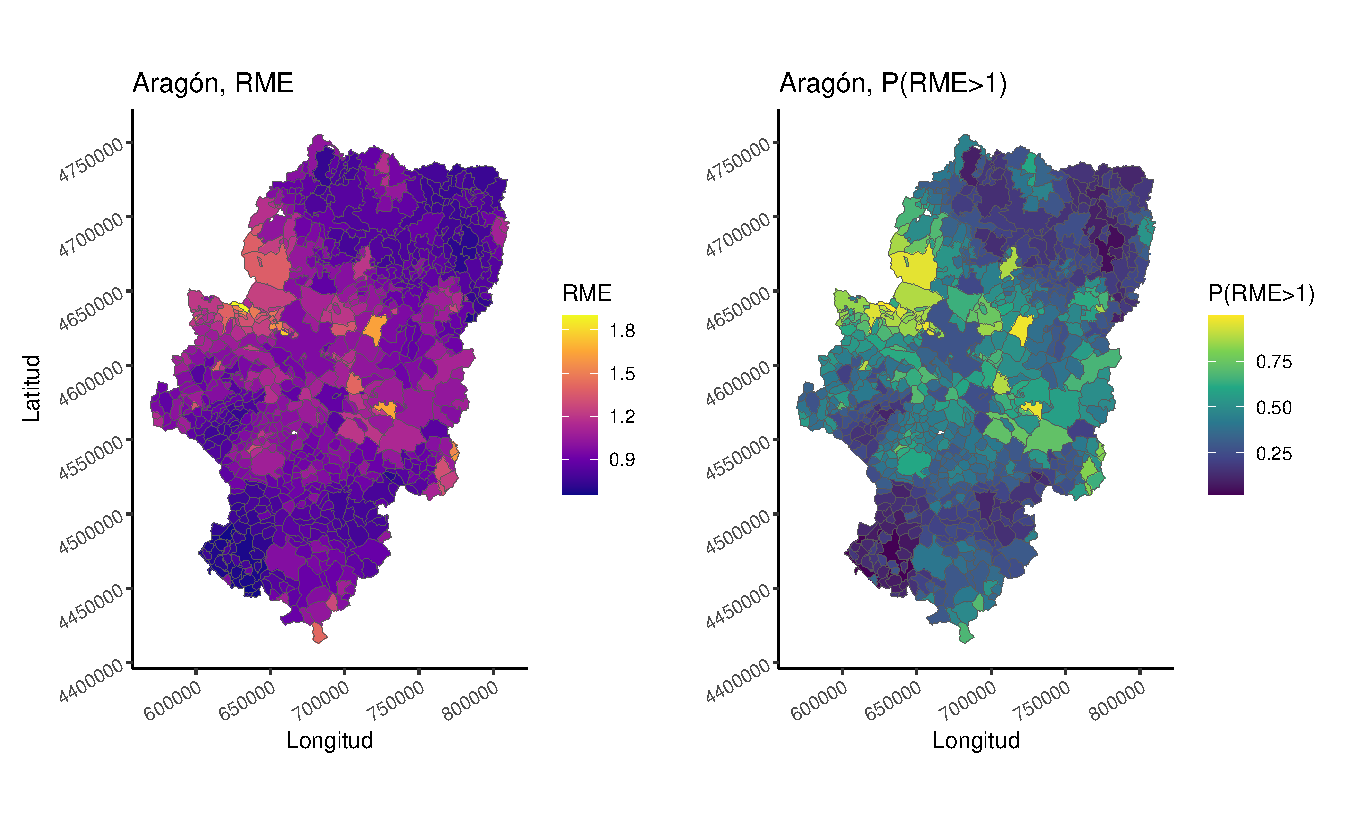
\includegraphics{disease_mapping_files/figure-pdf/plot-1.pdf}
\end{center}




\end{document}
